\documentclass[12pt,journal,compsoc]{IEEEtran}
\usepackage[utf8]{inputenc}
\usepackage{url}
\usepackage[final]{pdfpages}
\usepackage{graphicx}
\graphicspath{ {.} }

\ifCLASSOPTIONcompsoc
  % IEEE Computer Society needs nocompress option
  % requires cite.sty v4.0 or later (November 2003)
  \usepackage[nocompress]{cite}
\else
  % normal IEEE
  \usepackage{cite}
\fi

% correct bad hyphenation here
\hyphenation{op-tical net-works semi-conduc-tor}

\begin{document}

\title{Application of Kernel Principal Component\\ Analysis for Gesture Recognition}

\author{Ryan~Zoeller}%

\IEEEtitleabstractindextext{%
\begin{abstract}
In this paper we examine the application of kernel principal component analysis
to trajectory-based gesture recognition. Several gesture normalization methods are
compared, and shown to be roughly equivalent in the non-degenerate case.
The degenerate case is shown to be solvable using proportional scaling.
Two gesture input methods are proposed, and the classification algorithm is shown
to be agnostic to the data source, with potential applications in training gesture
classification algorithms for use in foreign or unknown environments.
\end{abstract}}

\maketitle

\IEEEdisplaynontitleabstractindextext

\IEEEpeerreviewmaketitle

\IEEEraisesectionheading{\section{Introduction}\label{sec:introduction}}

\IEEEPARstart{I}{n} many control applications it is desirable to
interact with a system without the use of tactile input such as buttons
or switches, or without being in direct contact. These situations often
arise in environments inherently hostile to traditional human-computer or
human-robot interaction methods, such as underwater. The nature of these
environments may rule out verbal communication mechanisms, necessitating
a visual control scheme. 
\par
In these circumstances, gestures can provide a flexible and expressive
vocabulary for conveying information. Gesture-based control has several
advantages over other control mechanisms: no complex hardware beyond a visual
camera is typically needed, a potentially unlimited number of gestures may
be learned by a system, and communication through hand gestures is innate
to humans. Unfortunately, the accurate classification of these gestures is
a nontrivial problem.
\par 
A simple machine learning algorithm is proposed using kernel principal
component analysis to separate the gestures, at which point a
$k$-nearest neighbors classifier can accurately identify the input.
Gestures are recorded as a series of time stamped points -- a normalization
process ensures that each gesture trajectory is scaled properly and interpolated
to contain the same number of points. We consider several normalization methods,
and analyze their performance across multiple data sets.
\par
The gesture recognition algorithm is experimentally shown to be agnostic of the
data source. Gesture trajectories are input via a mouse, and it is demonstrated
that these trajectories are sufficient to correctly classify trajectories input
through the use of a visual camera with blob tracking.
\par
The previously ignored degenerate case of one-dimensional gestures is considered,
and its tractability analyzed within the context of more normalization algorithms.


\section{Related Work} \label{relatedwork}

The notion of using gestures to interface with a control system is not
novel, especially in the context of human robot interaction. Typically,
points from a gesture are sampled temporally (e.g. through a camera) to
form a trajectory, and this trajectory is normalized before being compared
with known trajectories.
\par
Xu, Dudek, and Sattar propose augmenting an existing robotics control scheme
with gesture recognition~\cite{xu08}, in the domain of underwater robot control.
An iterative closest point approach was proposed, which attempts to
map sampled points from a given gesture to points in known gestures.
The mapping process uses Euclidean distance to find the nearest point
in the other gesture, with a penalty for deviating temporally beyond a given tolerance.
Trajectories are normalized along the axis of the principal eigenvector,
as well as temporally to a unit time.
\par
An alternate algorithm for performing gesture recognition is proposed by
Ramírez-Giraldo et al., which uses kernel-based method to separate
gestures for classification~\cite{giraldo12}. Kernel principal component analysis~(KPCA)
is applied to a trajectory sampled using a RGBD sensor, using a linear
combination of Gaussian radial basis functions as the kernel.
Trajectories are physically normalized to a unit height and width, as well
as temporally to a unit time.


\section{Methodology}

\subsection{Motivation}

This work is largely motivated by shortcomings in existing gesture recognition methods
which may cause some gestures to be ill-classified. The gesture recognition algorithms
proposed by Xu, Dudek, and Sattar~\cite{xu08} and Ramírez-Giraldo et al.~\cite{giraldo12}
both fail to classify degenerate cases properly: trajectories which are largely linear
or otherwise one-dimensional lose their orientation information, which prevents the use
of directed lines as gestures. The former reorients gestures such that their principal
eigenvectors are aligned in a uniform direction -- in the case of a line, all orientation
information will be discarded as the eigenvector's direction follows that of the line.
In the latter, the trajectory is normalized non-uniformly across the two observed physical
dimensions -- this effectively diagonalizes all lines which do not align perfectly to an axis.
\par
The motivation for using the kernel principal component analysis approach suggested by
Ramírez-Giraldo et al.~\cite{giraldo12} is its large number of other applications and
free accessibility. KPCA's ease of use was demonstrated by Raschka~\cite{raschka14} on
miscellaneous data, and their work served as a concrete foundation to build the multi-kernel
representation for classifying trajectories off of.


\subsection{Gesture shape}

The choice of gestures for an application is largely context dependent -- in some systems,
a large vocabulary may be required to accurately express all possible actions or objects.
In others, a smaller vocabulary may be used in combination with some sort of gesture composition.
In any case, the variation between unique gestures should be sufficiently large such that
both the human actor and classification algorithm can reliably reproduce and identify the gesture.
\par 
Two sets of gestures were chosen to test the classification algorithm, with the goal of covering
a broad range of potential use cases. The first set contains six capital letters chosen from
the English alphabet -- L, N, O, R, S, and W -- which were chosen due to their lack of ambiguity.
This set of symbols is a strict superset of that used by Ramírez-Giraldo et al.~\cite{giraldo12}.
\par
The second set of symbols was chosen to reflect the degenerate case in alternate gesture
recognition algorithms: eight lines were used, one corresponding to each cardinal direction
and the intermediate directions lying halfway in between them. In both implementations
discussed in section~\ref{relatedwork}, members of this set would not be properly classified
in all cases.

\subsection{Agnosticism to gesture source}

\begin{figure}
	\centering
	\includegraphics[height=7cm]{KPCAFlow}
	\caption{Gesture recognition process}
    \label{fig:KPCAFlow}
\end{figure}

The proposed gesture classification algorithm operates in several phases, as shown in
Figure~\ref{fig:KPCAFlow}. Notably, the trajectory normalization and KPCA processes are
not inherently aware of the source of the trajectory. As a result, it is possible to
have multiple data input sources use the same underlying classification algorithm.
Two gesture tracking frontends were created to test this principle: a cursor tracking
application and a camera-based blob tracking application.


\section{Trajectory normalization approach}

\subsection{Non-temporal interpolation strategy} \label{timeinvariant}

With time based interpolation, such as that used by Ramírez-Giraldo et al.~\cite{giraldo12},
temporal pauses or significant speed changes can significantly impact the resulting normalized
trajectory. Consider a trajectory drawn perfectly (i.e. that matches training data exactly),
except the operator pauses for a period of time at the start of the gesture. Under a time based 
interpolation method, every resampled point will be significantly shifted from the expected
location, which may result in an incorrect classification.
\par
There are several ways to mitigate this effect. When constructing training data, the speed and pauses
in a gesture could be intentionally varied, with the goal of anticipating where an operator may pause
or change speeds. Unfortunately, this requires some knowledge of the frontend environment -- what is the
maximum percentage of a gesture that an operator may spend (or appear to spend, due to tracking error) on
any section of the gesture? It also increases the variance of the gesture, potentially reducing its
separability with respect to other gestures.
\par
Xu, Dudek, and Sattar~\cite{xu08} provide an alternate approach, which removes points that are clustered
together and are matching with the same point in the training data. This completely removes the effect of
pausing, but is not immediately applicable to a kernel-based approach.
\par
A third option, which is tested, is to interpolate based on distance instead of time. That is, the
total length of the trajectory is calculated with Equation~\ref{distanceinterpolation}, and points
are sampled uniformly from this physical duration as opposed to the temporal duration.
This removes the temporal aspect of the gesture entirely, which may be undesirable in some cases.
It also fails in the case of high sampling error -- although an operator may not be moving,
it is possible that sampling noise will make the distance between identical points non-zero.

\begin{equation} \label{distanceinterpolation}
\textrm{Traj. Length} = \sum_{i=1}^{n-1}{\sqrt{(x_i - x_{i+1})^2 + (y_i - y_{i+1})^2}}
\end{equation}

\subsection{Non-linear interpolation strategy}

Linear interpolation is both incredibly fast and incredibly simple. These benefits come at 
the cost of sampling from a $C^0$ continuous function. The function produced by linear
interpolation effectively can change velocity and acceleration instantaneously, unlike
the physical system the trajectory represents.
\par
To more closely model the physical system the trajectory is derived from, a cubic-spline based
interpolation approach can be used. Here, samples are taken from a $C^2$ continuous function,
which should more accurately reflect the underlying gesture, at the price of increased computation.
The `not-a-knot' end condition is used when interpolating.
\par
As no elementary closed form exists in general for the length of a parametric function, a
length based approach such as the one described in section~\ref{timeinvariant} is not considered
for non-linear interpolation.

\subsection{Uniform scaling strategy}

Both implementations discussed in section~\ref{relatedwork} use non-uniform
physical scaling to normalize trajectories. This increases the similarity of
gestures which are drawn slightly in the incorrect proportion, which is
desirable, in general, for finding a match. Unfortunately, this also has the
effect of causing gestures with wildly different proportions but a similar
underlying shape to be stretched to the same representation.
\par
For example, consider a long, thin rectangle and a square. Scaled proportionally,
other rectangles and squares will match to the appropriate shape. When scaled
non-uniformly, the rectangle will be compressed and stretched to a square.
\par
A proportional normalization method is proposed that scales trajectories such
that the axis with the largest range is scaled to uniform size. The other axis
is scaled by the same factor.


\section{Results}

\subsection{Non-degenerate classification}

A total of 720 trajectories across the six gestures (L, N, O, R, S, W) were
recorded by six subjects using the cursor tracking front end. The trajectories
were normalized using a given trajectory normalization approach, and partitioned
into buckets of 240 elements at random. A kernel principal component analysis
was performed on one bucket, and the other buckets classified against the first.
This process was repeated for each bucket and the number of failures averaged;
the entire procedure was then repeated for each trajectory normalization approach.
The results are shown in Table~\ref{tab:nondegenerate}.

\begin{table}[!tp]
\centering
\caption{Classification of mouse-derived trajectories against one third of mouse-derived samples}
\label{tab:nondegenerate}
\begin{tabular}{|c|c|c|}
\hline
\begin{tabular}[c]{@{}c@{}}Normalization \\ strategy\end{tabular}                & \begin{tabular}[c]{@{}c@{}}Average classification\\ failures (maximum 480)\end{tabular} & \begin{tabular}[c]{@{}c@{}}Success\\ rate\end{tabular} \\ \hline
\begin{tabular}[c]{@{}c@{}}Linear (time),\\ non-uniform scaling\end{tabular}     & 0.67                                                                                    & 99.9\%                                                 \\ \hline
\begin{tabular}[c]{@{}c@{}}Linear (time),\\ uniform scaling\end{tabular}         & 1.33                                                                                    & 99.7\%                                                 \\ \hline
\begin{tabular}[c]{@{}c@{}}Linear (distance),\\ non-uniform scaling\end{tabular} & 0.67                                                                                    & 99.9\%                                                 \\ \hline
\begin{tabular}[c]{@{}c@{}}Linear (distance),\\ uniform scaling\end{tabular}     & 1.33                                                                                    & 99.7\%                                                 \\ \hline
\begin{tabular}[c]{@{}c@{}}Cubic spline,\\ non-uniform scaling\end{tabular}      & 1.33                                                                                    & 99.7\%                                                 \\ \hline
\begin{tabular}[c]{@{}c@{}}Cubic spline,\\ uniform scaling\end{tabular}          & 0.67                                                                                    & 99.9\%                                                 \\ \hline
\end{tabular}
\end{table}

The high classification accuracy can be visually confirmed by examining the kernel
similarity matrix of all 720 trajectories, as shown in Figure \ref{fig:kernelsimilaritymatrix}
for the distance-based linear interpolation strategy.
It is observed that the diagonal has significantly higher intensity than other areas of
the matrix. This indicates that each group of trajectories is very similar to itself, and
does not resemble trajectories associated with other gestures.

\begin{figure}[htbp]
	\centering
	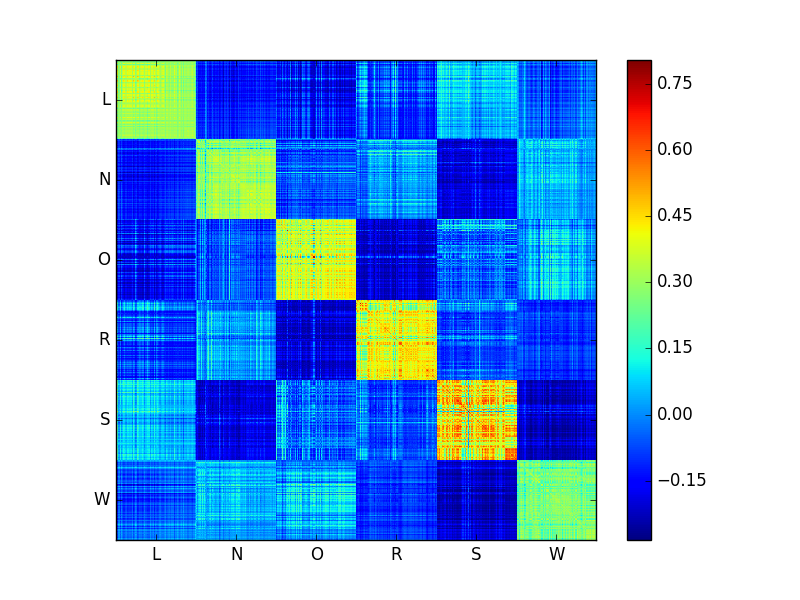
\includegraphics[trim={2cm 0 1cm 0},clip,width=10cm]{KernelSimilarityMatrix}
	\caption{Kernel similarity matrix under time invariant linear interpolation}
    \label{fig:kernelsimilaritymatrix}
\end{figure}

A total of 120 trajectories were recorded using a vision-based blob tracker. The
results of classifying this dataset against the 240 trajectory buckets described above
can be seen in Table~\ref{tab:nondegeneratekinect}.

\begin{table}
\centering
\caption{Classification of vision-derived trajectories against one third of mouse-derived samples}
\label{tab:nondegeneratekinect}
\begin{tabular}{|c|c|c|}
\hline
\begin{tabular}[c]{@{}c@{}}Normalization \\ strategy\end{tabular}                & \begin{tabular}[c]{@{}c@{}}Average classification\\ failures (maximum 120)\end{tabular} & \begin{tabular}[c]{@{}c@{}}Success\\ rate\end{tabular} \\ \hline
\begin{tabular}[c]{@{}c@{}}Linear (time),\\ non-uniform scaling\end{tabular}     & 2.67                                                                                    & 97.8\%                                                 \\ \hline
\begin{tabular}[c]{@{}c@{}}Linear (time),\\ uniform scaling\end{tabular}         & 0.87                                                                                    & 99.3\%                                                 \\ \hline
\begin{tabular}[c]{@{}c@{}}Linear (distance),\\ non-uniform scaling\end{tabular} & 0.00                                                                                    & 100.0\%                                                \\ \hline
\begin{tabular}[c]{@{}c@{}}Linear (distance),\\ uniform scaling\end{tabular}     & 0.08                                                                                    & 99.9\%                                                 \\ \hline
\begin{tabular}[c]{@{}c@{}}Cubic spline,\\ non-uniform scaling\end{tabular}      & 2.00                                                                                    & 98.3\%                                                 \\ \hline
\begin{tabular}[c]{@{}c@{}}Cubic spline,\\ uniform scaling\end{tabular}          & 0.33                                                                                    & 99.7\%                                                 \\ \hline
\end{tabular}
\end{table}


\subsection{Degenerate classification}

\begin{table}[htbp]
\centering
\caption{Classification of mouse-derived degenerate trajectories against one half of mouse-derived samples}
\label{tab:degenerate}
\begin{tabular}{|c|c|c|}
\hline
\begin{tabular}[c]{@{}c@{}}Normalization \\ strategy\end{tabular}                & \begin{tabular}[c]{@{}c@{}}Average classification\\ failures (maximum 120)\end{tabular} & \begin{tabular}[c]{@{}c@{}}Success\\ rate\end{tabular} \\ \hline
\begin{tabular}[c]{@{}c@{}}Linear (time),\\ non-uniform scaling\end{tabular}     & 46.13                                                                                   & 61.6\%                                                 \\ \hline
\begin{tabular}[c]{@{}c@{}}Linear (time),\\ uniform scaling\end{tabular}         & 1.00                                                                                    & 99.2\%                                                 \\ \hline
\begin{tabular}[c]{@{}c@{}}Linear (distance),\\ non-uniform scaling\end{tabular} & 52.63                                                                                   & 56.1\%                                                 \\ \hline
\begin{tabular}[c]{@{}c@{}}Linear (distance),\\ uniform scaling\end{tabular}     & 26.00                                                                                   & 78.3\%                                                 \\ \hline
\begin{tabular}[c]{@{}c@{}}Cubic spline,\\ non-uniform scaling\end{tabular}      & 46.50                                                                                   & 61.3\%                                                 \\ \hline
\begin{tabular}[c]{@{}c@{}}Cubic spline,\\ uniform scaling\end{tabular}          & 2.25                                                                                    & 98.1\%                                                 \\ \hline
\end{tabular}
\end{table}

A total of 320 trajectories across the eight lines following the cardinal and intermediate
directions were recorded by two subjects using the cursor tracking front end. The trajectories
were normalized using a given trajectory normalization approach, and partitioned
into buckets of 160 elements at random. A kernel principal component analysis
was performed on one bucket, and the other bucket classified against the first.
This process was repeated for both buckets and the number of failures averaged;
the entire procedure was then repeated for each trajectory normalization approach.
The results are shown in Table~\ref{tab:degenerate}.
\par
The kernel similarity matrices for the degenerate case explain why the success rates are so bad in
the case of non-uniform scaling. When uniform scaling is applied, as shown in
Figure~\ref{fig:kernelsimilaritymatrixdegenerategood}, the diagonal remains well structured, as
was the case with the non-degenerate gestures. When the gestures are scaled non-uniformly,
diagonalization of the trajectories occurs, resulting in the similarity matrix shown in
Figure~\ref{fig:kernelsimilaritymatrixdegeneratebad}. It is immediately clear that many lines on
the cardinal directions have become aligned with the intermediate directions.

\begin{figure}[tbp]
	\centering
	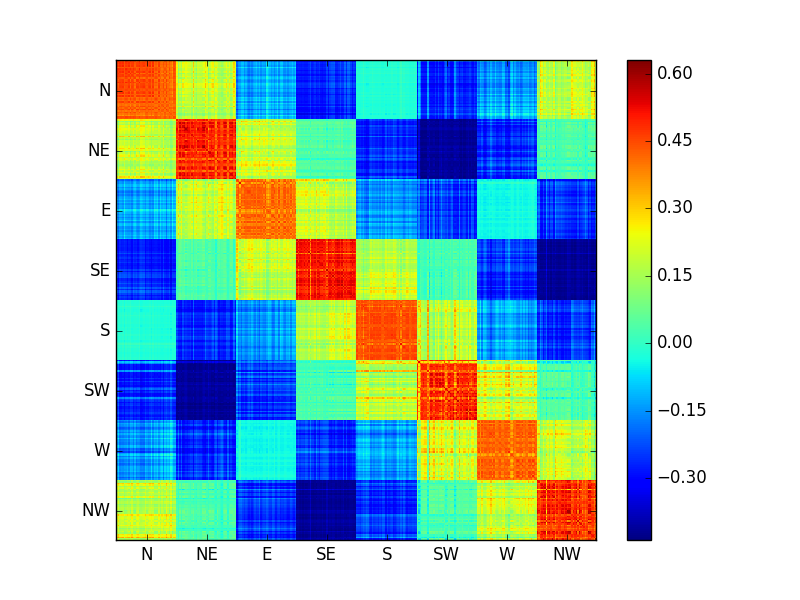
\includegraphics[trim={2cm 0 1cm 0},clip,width=10cm]{KernelSimilarityMatrixDegenerateGood}
	\caption{Kernel similarity matrix under linear interpolation with uniform scaling}
    \label{fig:kernelsimilaritymatrixdegenerategood}
\end{figure}

\begin{figure}[tbp]
	\centering
	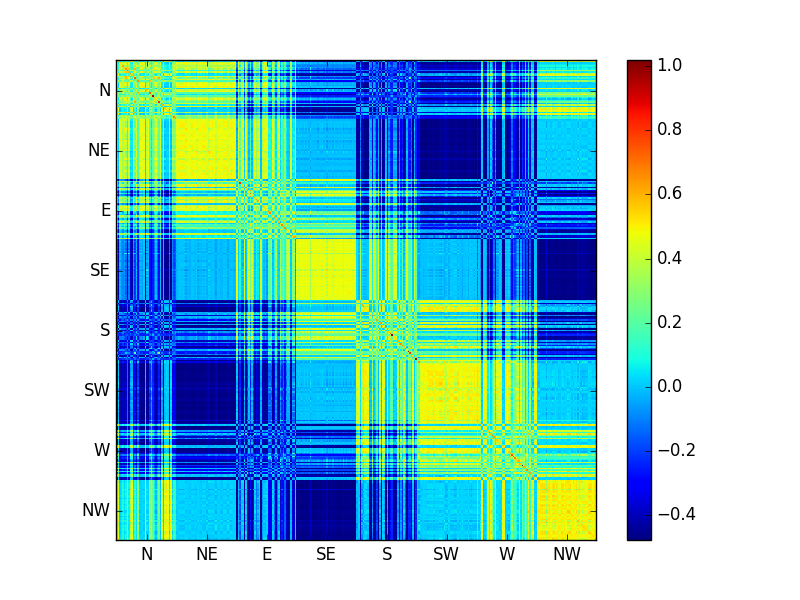
\includegraphics[trim={2cm 0 1cm 0},clip,width=10cm]{KernelSimilarityMatrixDegenerateBad}
	\caption{Kernel similarity matrix under linear interpolation with non-uniform scaling}
    \label{fig:kernelsimilaritymatrixdegeneratebad}
\end{figure}

The first three principal components are enough to see the diagonalization phenomena.
Figure~\ref{fig:principalcomponentsdegenerategood} shows the the uniformly scaled projection;
each gesture is clustered distinctly from all other gestures, and there are eight well defined groups.
Figure~\ref{fig:principalcomponentsdegeneratebad} shows the the non-uniformly scaled projection;
there are four primary groups, with significant noise in between the the clusters. Unlike in the 
uniformly scaled case, there is no easy way to partition this space into eight gestures.

\begin{figure}[tbp]
	\centering
	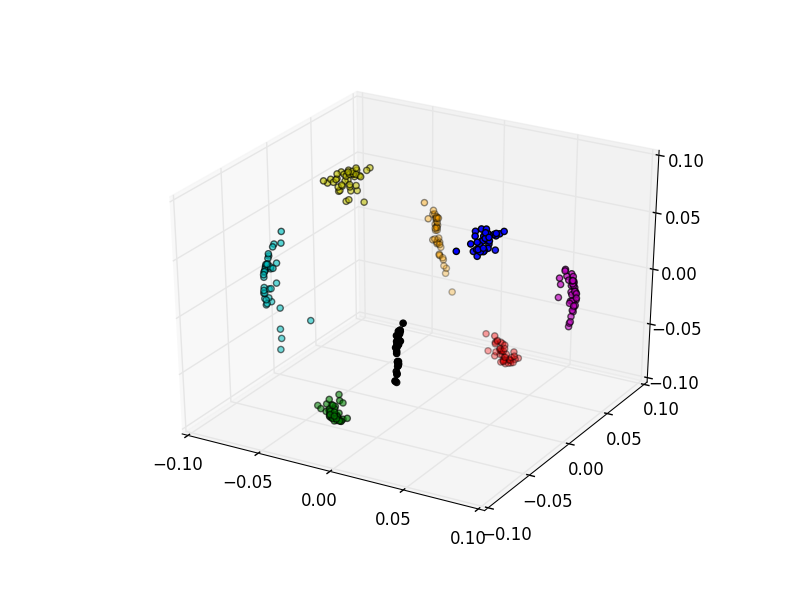
\includegraphics[trim={2cm 0 1cm 0},clip,width=10cm]{PrincipalComponentsDegenerateGood}
	\caption{First three principal components under linear interpolation with uniform scaling}
    \label{fig:principalcomponentsdegenerategood}
\end{figure}

\begin{figure}[tbp]
	\centering
	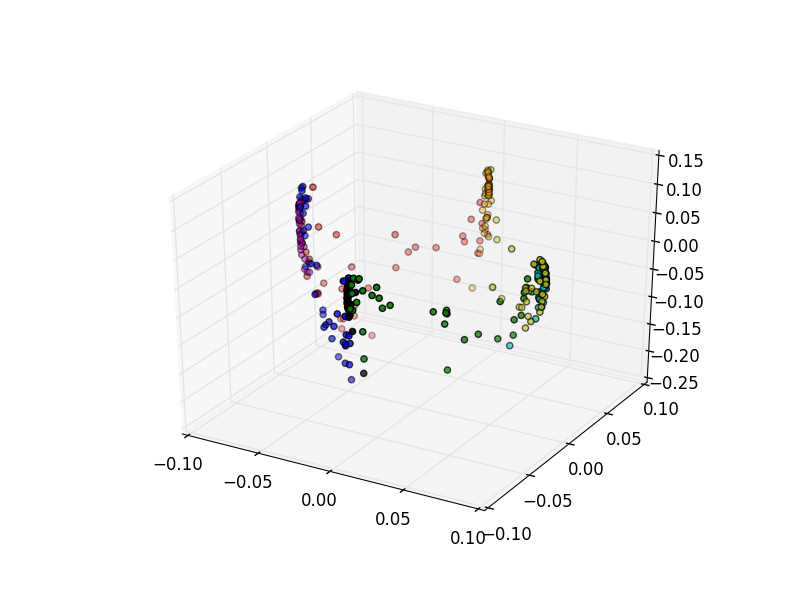
\includegraphics[trim={2cm 0 1cm 0},clip,width=10cm]{PrincipalComponentsDegenerateBad}
	\caption{First three principal components under linear interpolation with non-uniform scaling}
    \label{fig:principalcomponentsdegeneratebad}
\end{figure}


\section{Conclusion}

\subsection{Analysis}

Using kernel principal component analysis is a viable approach for gesture recognition. 
However, there is no clear consensus on which trajectory normalization method is best;
the normalization methods most accurate for classifying non-degenerate gestures are not
the same as the normalization methods most accurate for classifying degenerate gestures.
\par
In the non-degenerate case linear, time invariant interpolation performed extremely well,
including when comparing to gestures tracked using an alternate mechanism. The pauses and
speeds with which an operator can trace a gesture will vary significantly between media, which
makes time a poor indicator to rely on when crossing between applications. However linear,
time invariant interpolation performed poorly in the degenerate case, including when
uniform scaling was used.
\par
When attempting to classify degenerate trajectories (Table \ref{tab:degenerate}),
the uniformly scaling time based linear interpolation and cubic spline interpolation
methods performed extremely well.
\par
The agnosticism of the underlying KPCA classifier to the trajectory source was
largely confirmed. This has potential applications in creating training datasets --
it is not necessary to duplicate the production environment in order to train the model.
This significantly impacts non-traditional control applications, such as the underwater
human-robot interaction work done by Xu, Dudek, and Sattar~\cite{xu08}, as it may not
be necessary to replicate either the robot or underwater environment to enable new
functionality.

\subsection{Future work}

The iterative closest point method suggested by Xu, Dudek, and Sattar~\cite{xu08}
handles the case of ill-defined trajectory bounds, by discarding points on the ends
of trajectories that do not match to known models. Further investigation of this
approach's relevance to a kernel based approach is desirable.


\nocite{*}
\bibliographystyle{plain}
\bibliography{bibliography.bib}{}

\clearpage
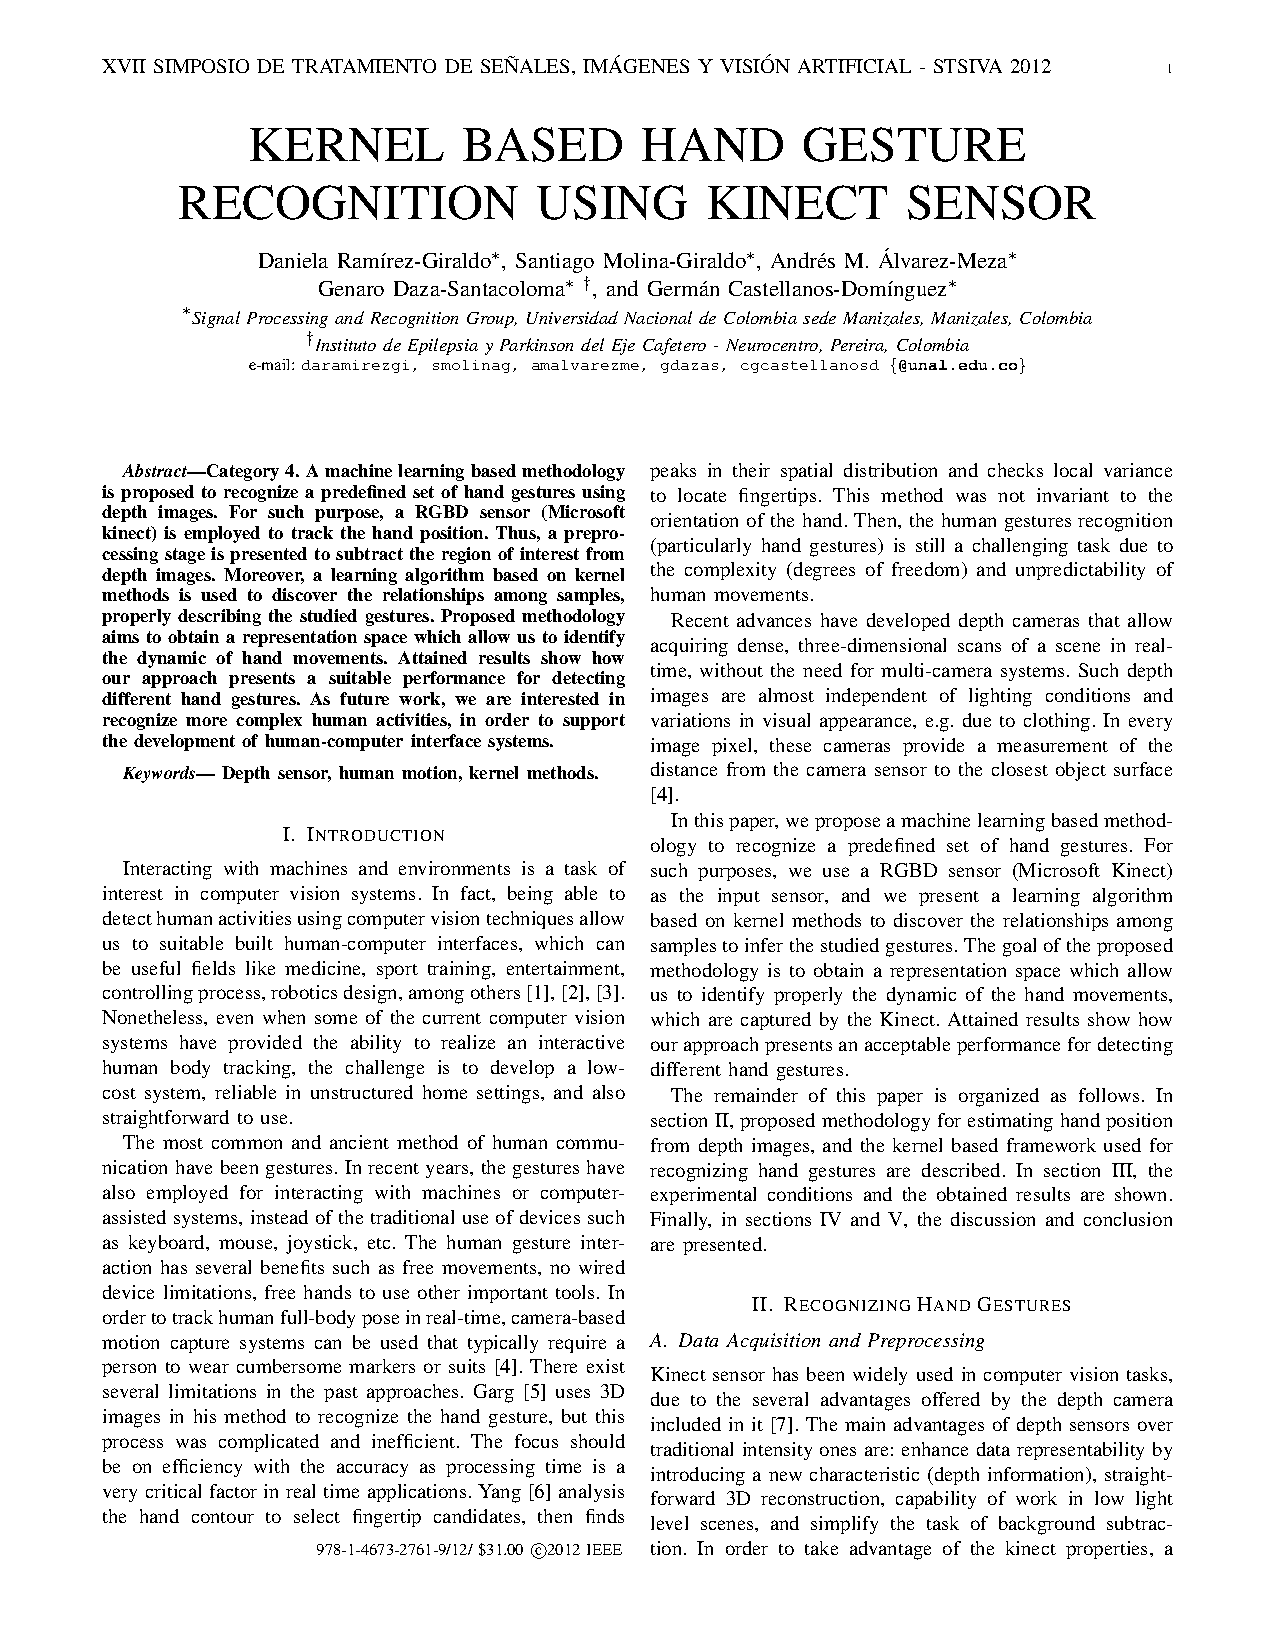
\includepdf[pages=-]{ramirez-giraldo12.pdf}
\clearpage
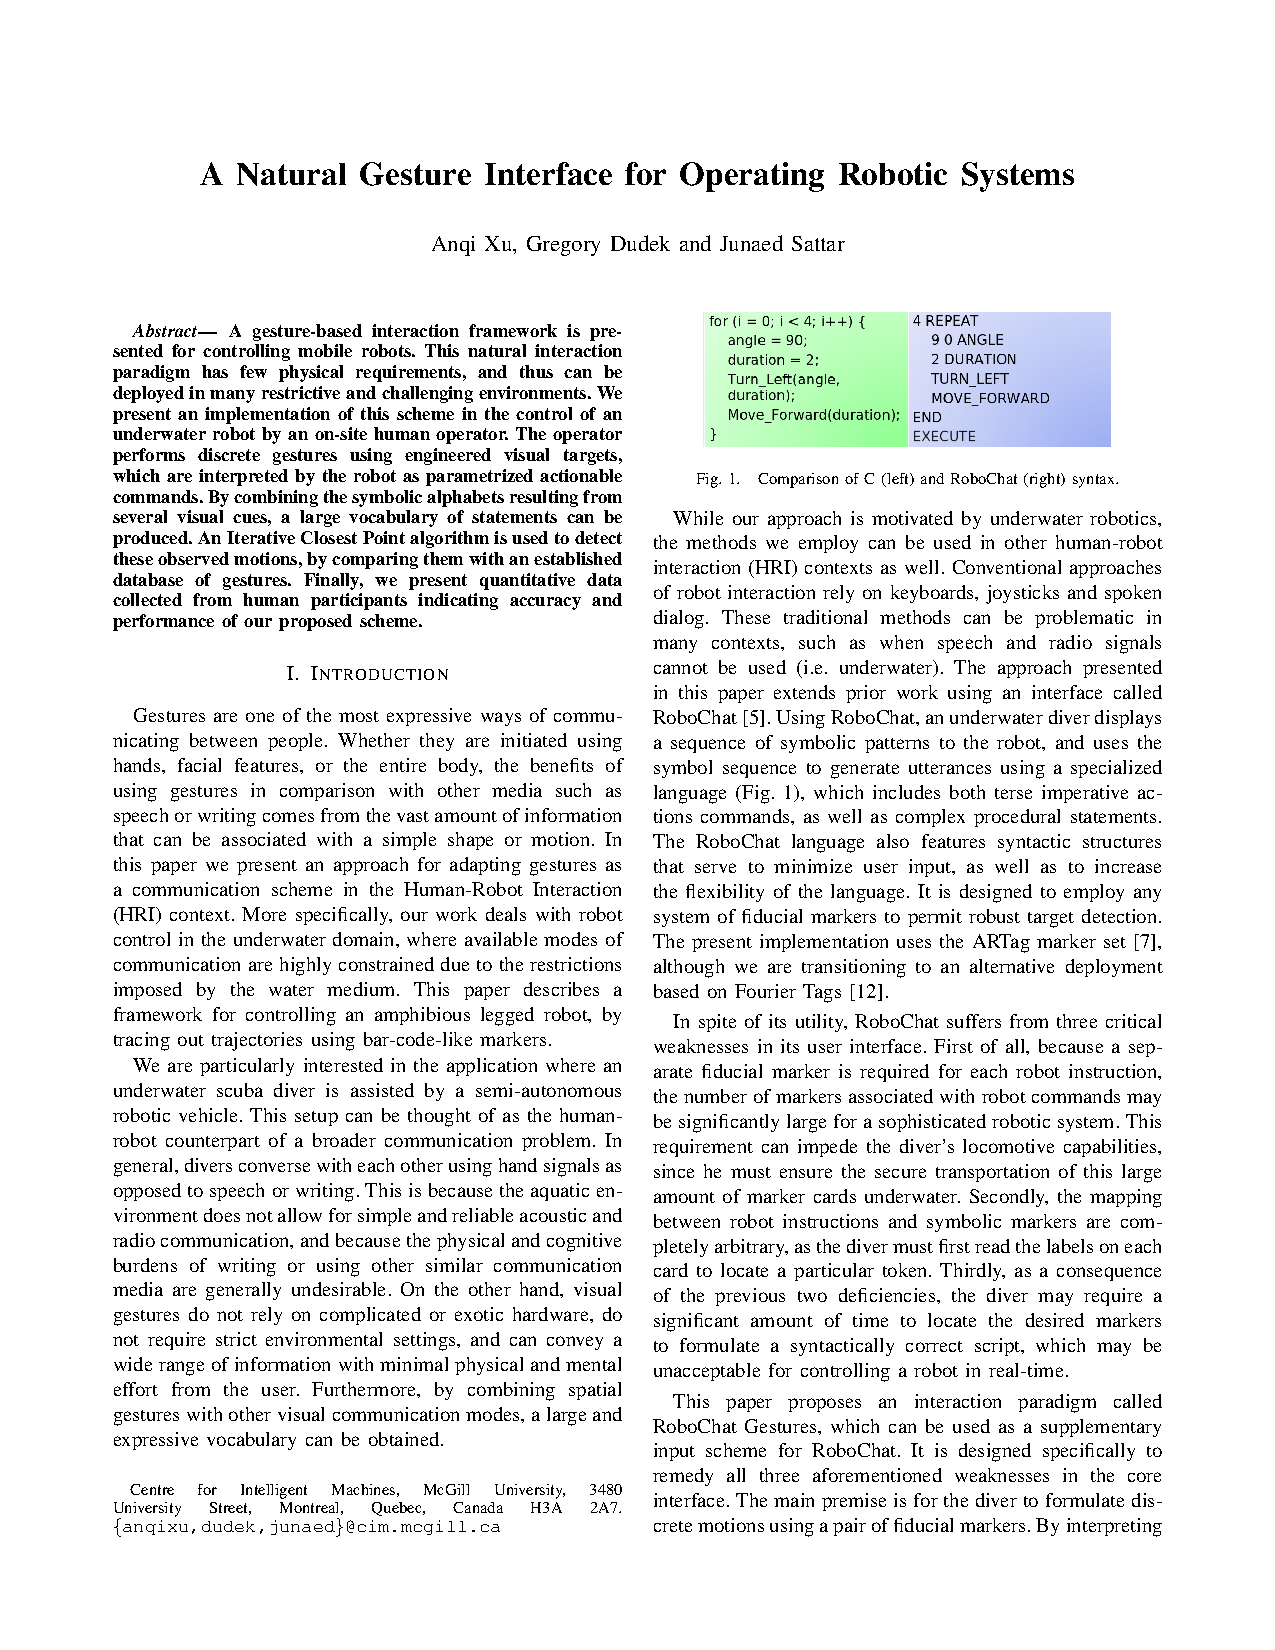
\includepdf[pages=-]{xu08.pdf}


\end{document}


